\documentclass[12pt]{article}
\usepackage{url}
\usepackage[authoryear,round]{natbib}
\usepackage{graphicx} 

\title{Outline flowCore paper}

\author{Florian Hahne*\\
  Nolwenn LeMeur*\\
  Byron Ellis\\
  Ryan Brinkman\\
  Perry Haaland\\
  Errol Strain\\
  Deepayan Sarkar\\
  Josef Spidlen\\
  Robert Gentleman
 }

\begin{document}

\maketitle

\section*{Introduction}
During the last several years, automation technologies have been developed
that enable the use of flow cytometry high content screening (FC-HCS)
to generate large, complex datasets in both basic and clinical research
applications \citep{brinkman2007hcf}. A
serious bottleneck in the intepretation of existing studies and the application of
FC-HCS to even larger, more complex problems is that data management
and data analysis methods have not advanced sufficiently far from the
methods developed for 
traditional applications of flow cytometry (FCM) to small-scale, tube-based
studies. 

Some of the consequences of this lag in development are difficulties in 
maintaining the integrity and documentation of extremely large datasets,
assessing measurement quality, developing validated assays, assessing the
accuracy of gating techniques, automating complex gating strategies, and
aggregating statistical results across large study sets for further analysis.
Among the most serious consequences of the current situation is, however, 
that it is very difficult for new analysis
approaches to find there way into standard practice. We believe that
this barrier to the development and dissemination of new analysis methods
is one of the fundamental restraints on the
future expansion of FC-HCS in both clinical and research applications.

In this paper, we describe a set of flexible and well
structured computational tools to efficiently analyze
FC-HCS. This set of tools is based on the open source statistical
software R, in conjunction with the Bioconductor Project. Our intent
is to provide a shared research platform that enables
bioinformaticians, computer scientists, and statisticians to work
collaboratively with biologists and clinicians to develop novel methods \citep{lizard2007fca} for FCM
data analysis. A critical component of this approach is the development and implementation
of standards that will facilitate the adoption of these methods
by both the larger research community and commercial software vendors.
Consequently, we are optimistic that this software platform will play a
critical role in addressing the bottlenecks described above that limit
further advances in the application of FC-HCS.

The computational tools we have developed are distributed in the R 
software language (www.r-project.org) as the Bioconductor
(www.bionductor.org) package flowCore. flowCore is a freely available, highly
functional and extensible FCM data analysis platform that 
enables researchers to efficiently handle FC-HCS data and encourages open
development of tools for their coherent analysis. Among the issues
addressed by flowCore are computationally efficient data structures and
a range of specialized methods for compensation, transformation, and gating. 
flowCore runs on Windows, Mac OS X and Linux/Unix operating
systems.  In this paper, we describe the functionality and methods underlying flowCore, 
and provide examples of their use.


\subsection*{R and Bioconductor}
R is a robust statistical programing environment which offers a wide
range of statistical and visualization methods developed for various
fields of application. In addition, R is an open source research %already mentioned R, and by extention flowCore open source
platform that bioinformaticians, computer scientists, and
statisticians routinely use to develop novel tools and methodology for
statistical data analysis. For biological applications, the
Bioconductor project has become the standard toolset
\citep{gentleman2006bos} to process data spanning a diversity of
research fields from genomics to proteomics to cell
biology. It is particularly geared towards the analysis of large
numeric datasets that typically arise from high throughput experiments
such as microarray gene expression analysis or FC-HCS. A shared
platform has proven to be particularly beneficial for the development of
analysis routines for microarray gene expression data, and by today
many of these early innovations have been incorporated into commercial
software products, thus greatly improving the quality of gene
expression data analysis. 
%% NLM: that's probably the important point: platform for innovation rather than for standardization
Shared data structures have been shown to be
essential for such a collaborative effort. We envision a similar
paradigm for FC-HCS data. 


\subsection*{Existing data standards and conventions}
Currently, data from FCM experiments are stored in single files
according to the Flow Cytometry Standard (FCS) \citep{seamer1997pnd}.
%This standard attempts to capture much of the accompanying meta information, most of which is produced by the measurement instrument or has to be supplied manually by the operator upon experiment setup. - I believe FCS only tries to capture a subset of meta information
However, the recent
developments in high-throughput FCM are shifting the focus
of interest away from single-tube based measurements towards large and
complex experimental designs with dozens of co-variates and
influencing factors. Self-contained and self-reflective data
structures are a prerequisite to allow for coordinated analysis of
such experiments. Most of the currently available software solutions
offer only limited support for such structures, or make use of
containers like XML or binary storage formats that are designed
specifically for the mostly GUI-driven user interfaces and hence are
not easily amenable to programmatical access. In addition, the
closed-source nature of %most of <can you think of an example that is not closed source?>
these products makes it impractical to
connect to and integrate the data into an analysis pipeline.

Traditionally, the majority of FCM experiments have been analyzed
manually by direct data inspection in one or two dimensions, or by
very basic comparisons of summary statistics. We believe that these
approaches do not fully address the highly complex nature of FCM data,
in particular, they discard many of the fundamental aspects of the
data, such as its underlying distribution and its high-dimensional
nature. In addition, the subjective character of manual analyses are a
major obstacle to reproducibility. For FC-HCS data, unassisted manual
inspection has become time consuming and labor intensive, and robust
statistical methods need to be developed to point the investigator to
the interesting aspects of the data or to potential problems. While
the expert knowledge of immunologists and researchers remains crucial
for the understanding of FCM data, we believe that close collaboration
with other research fields such as statistics and computer science can
greatly improve the relevance of FCM in today's high-throughput
paradigm.

These issues are currently being addressed by emerging new flow
cytometry data standards developed in collaboration with the ISAC Data
Standards Task Force.  For example, the Gating-ML Candidate Recommendation (CR)
represents a proposal on how to form unambiguous XML-based gate
definitions, which can facilitate the interchange and validation of
data between different software packages with the potential of
significant increase of hardware and software interoperability. Gates
may be ordered into a hierarchical structure to describe a gating
strategy. They may be applied on parameters as in FCS files or on
transformed parameters as described by an explicit parameter
transformation. 
%% I find the previous sentence redundant - 
%% They may be applied on raw or transformed parameters
%% EAS: I don't believe the previous sentence is required.
This enables the encoding of a simple analytical workflow, in a way
that allows us to reconstruct the analysis programmatically.

The flowCore framework presented here offers import functionality for
raw data FCS files along with their complete set of file-specific meta
information (Figure~\ref{fig1:FrameWork}). Moreover, it is a software
implementation of the Gating-ML CR, which opens the possibility to
integrate flowCore in existing workflows and to communicate with
every other FCM tool that adheres to the proposed
standard. Adherence to standards also plays a critical role in the ability
of new methods based on flowCore to find there way back into the
standard practices for FCM data analysis.

flowCore is not a GUI-driven software, and all operations are done
using a command line interface. Conceptually, it is possible to add a
more elaborate user interface on top of that, however the focus is on
a programmatic approach to enable the convenient development of novel
analysis methods and automation of complex analysis approaches. By taking the
burden of data management from the programmer, and by providing well-defined 
APIs and a structured class
hierarchy, it is possible to readily test new ideas and to easily
extend the framework's functionality. %Both the underlying R and
%Bioconductor software and flowCore itself are open source and open %already mentioned its open source
%development projects, thus community involvement in the developing
%process is highly appreciated. 



\section*{Basic data structures}
\subsection*{Flow Frame}
flowCore's primary task is the representation and basic manipulation
of FCM data. This is accomplished through a data model very
close to that adopted by other Bioconductor packages used for gene
expression analysis, and thus familiar to most Bioconductor
users. Similar to any other FCM data analysis tool, the basic unit of organization
in flowCore is a collection of events. We call the structure that hold
this data a flow frame. All relevant information for the collection
are stored along with the matrix of raw data values and can be
accessed programmatically. Most commonly, these are descriptors of the
stains used in the experiment and the respective measurement channels,
information about compensation performed at the instrument side and
any additional keywords the user deems to be important to annotate the
data. A number of quality checks are performed during the creation of
a flow frame to ensure data integrity. There is an extended interface
that allows for the standardized interaction with the flow data, thus
enabling the development of more specialized tools for specific tasks
of the data analysis process that all share a common Application Program Interface (API).

\subsection*{Flow Set}
In high-throughput FCM, many of the analysis tasks need to be
performed consistently across multiple flow measurements, hence we
introduce the concept of a collection of flow frames called a flow
set. Flow sets store the relevant information associated with each
individual frame such as descriptions of the samples or the treatment
to which a sample was subjected, and they manage the consistent
application of operations on the individual flow frames. The burden of
keeping score of the annotation is shifted from the user to the
infrastructure, thus reducing the risk of common errors % (\textit{i.e.}, example of an error ) 
that occur when using more or less ad hoc spreadsheets that
lack a controlled structure. There is no native ordering
to a flow set, which in a way reflects the still predominant
application of tube-based experiments rather than experiments
that depend on automated sample acquisition using a plate-based platform. 
%% EAS: I don't think the previous sentence is required. Does it 
%% matter if the flowSet is ordered or not?

%However, the flow set structure can be
%readily extended to also accommodate such spatial information
%% EAS: The spatial aspect of plateCore is really secondary to having 
%% an easy, consistent way to manage and access the mulitplex annotation.
%% Also, it's important to have a standard format for the annotation if
%% we're trying to encourage collaboration. I haven't done it yet, but I 
%% intend to look into
%% into stealing the annotation implementation from CellHTS2 and
%% using it in plateCore.
However, the flow set structure can be readily extended to incorporate the
potentially complex annotation associated with large FC-HCS experiments. Access
to flowCore data structures and methods has already enabled the development of
new Bioconductor pacakges, such as plateCore, that faciliate the analysis of
plate-based FC-HCS data and make handling the annotation and processing
the data easier.

%\textit{(plateCore reference, Perry, Errol?)}.

%%Figure1 Diagram of the data structures and the basic operations
\begin{figure}
\centering
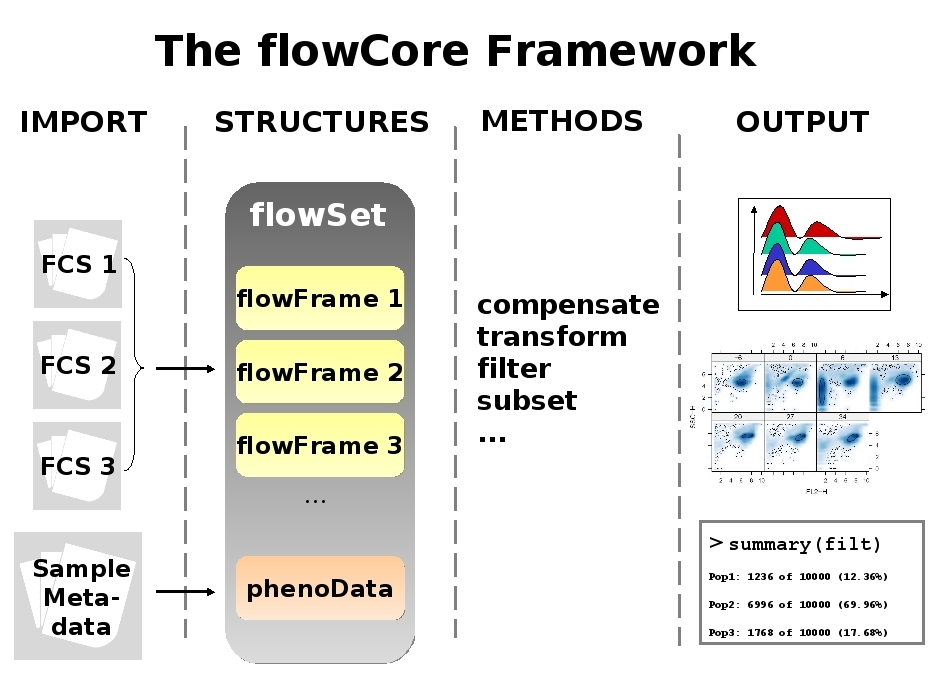
\includegraphics[width=0.9\textwidth]{Figure1-flowCoreFrameWork.jpg}
\caption{\label{fig1:FrameWork}{The flowCore frame work. For each
    experiment, FCS files, phenotypic and meta data is stored in a
    flow set. Each flow frame of a flow set corresponds to one FCS
    file. All basic operations (e.g., compensation, transformation,
    gating) can be applied on both single flow frames or entire flow
    set.}}
\end{figure}


\section*{Standard flow operations}
The basic operations in FCM analyses are typically the same: the data
need to be compensated (if not already done on the instrument side)
and transformed, and sup-populations of interest need to be selected
based on a set of (predominantly sequential) gates. All software
solutions for FCM analysis offer more or less elaborate support for
these kinds of operation, and most of them in an interactive,
GUI-driven interface. The approach we have taken in flowCore is to
abstractly describe these operations and build a set of tools to
perform them on both flow frames and flow sets. While transformation,
and to a certain extent compensation, are fairly routine operations
with only limited potential for improvement, being able to implement
new methodologies for gating of FCM data, and extending the
capabilities of flowCore through object oriented programming are
features that clearly sets our framework apart from other FCM analysis
tools. By factoring out as much of the bookkeeping as possible,
programmers can focus on the actual operations rather then having to
deal with the tedious details of data integration and
access. Third-party methods can act on their own as first-class
citizens in the analysis framework, without breaking the workflow or
the basic infrastructure. This design allows for the straightforward
extension of flowCore's capabilities, and has already fostered the
development of a number of valuable add-ons
\citep{lo2008agf,sarkar2008ufv} \textit{(plateCore}.




\subsection*{Transformation and compensation}
Data transformation is essential for both data visualization and
modelling \citep{lo2008agf}. The major transformations that are
routinely used in FCM analysis have been implemented in flowCore
(\textit{e.g.,} quadratic, log or arcsinh). Furthermore, the design of the R language makes
it easy to define arbitrary functions to apply to the data of
individual flow frames or entire flow sets, respectively. Compensation
is available for both flow frames and flow sets, and the software also
offers functionality to compute spillover or compensation matrices
from a set of appropriate compensation samples.



\subsection*{Gating}
In flowCore, gating operations are represented by classes that can be
extended in an object-oriented manner. Basic gate types such as
rectangular gates, ellipses and polygon gates are implemented as part
of the framework. In addition, we introduce the notion of data-driven
gates, or filters, for which the necessary parameters are computed
based on the properties of the underlying data, for instance by
modelling underlying data distribution or by density estimation. The
ability to programmatically access gates is a prerequisite for
automated or semi-automated gating. By utilizing a unified interface
for all different types of gates, the user is able to subset data sets
as well as to create summary statistics, like the proportions of
events falling in single gates or in the combinations of
gates. Complex combinations and hierarchies of gates can be captured
in objects of class filterSet, allowing to apply multi-step gating
strategies. The definition of gates in flowCore follows the Gating-ML
CR, thus any flowCore gating strategy can be reproduced by any other
software that also adheres to the standard.

\section*{Related flow packages}
In addition to the flowCore package that offers basic infrastructure,
we have implemented a range of additional Bioconductor packages that
are dedicated to more specific tasks of FCM data analysis
(Figure \ref{fig2:flowWheel}). The flowViz package provides
sophisticated data visualization tools, that make use of multivariate
trellis plotting. These functions can be used to quickly generate
customized plots for extended cytometry data sets for both direct data
inspection and quality control. The flowQ package offers more advanced
quality assurance (QA) methodology and a framework to create
interactive web-based reports of QA results. Most of flowUtil's
content deals with data import and output from and to flowCore and the
flow-cytometry specific standard markup languages. Finally, flowStats
provides statistical methods that are relevant in the context of flow
cytometry data analysis.


%\begin{figure}
%\centering
%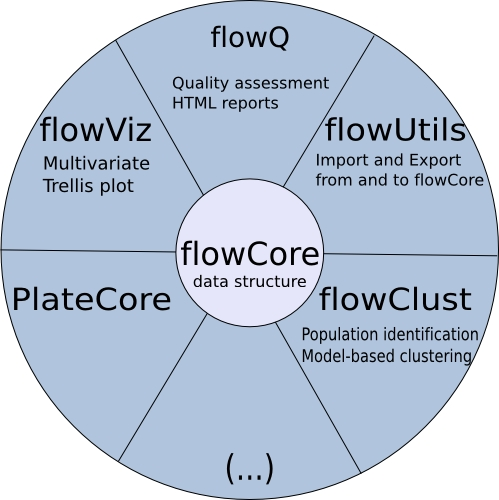
\includegraphics[width=0.6\textwidth]{Figure2-flowWheel-version4.jpg}
%\caption{\label{fig2:flowWheel}{flowCore and assoziated Bioconductor
%    packages: dedicated packages have been developed that utilize
%    flowCore’s data structures. flowViz is a data visualization
%    package; flowQ provides data quality assessment methods; flowUtils
%    contains interfaces for flow data, including xml parsers:
%    flowClust provides automated gating by model-based clustering.}}
%\end{figure}


\section*{Application}
The flowCore package has successfully been applied in the analysis of
several datasets \citep{gasparetto2004ice,brinkman2007hcf}, and
several other Bioconductor packages are making use of its code
base. As an example, \cite{lo2008agf} have recently developed an
automatic gating approach via robust model-based clustering using the
flowCore data model and infrastructure and implemented this in the
Bioconductor package flowClust. Another package (plateCore) providing
more specialized support for experiments conducted on microtitre
plates is under development. The documentation of all of flowCore's
features is beyond the scope of this publication, however additional
documentation and users guide information with programmatic examples
is available <here> . However, in the Supplementary Material to this
article we use a single example to demonstrate some of the software's
hallmarks, including the concept of data-driven automated gating, the
integration of existing software into the framework, and the
generation of publication-quality graphics for data visualization.

%% not sure about this next section vs. the use of Suuplementary material. Would it be useful/informative to show the code required to generate the plot? Otherwise I'm not sold that the next paragraph adds anything.

%% I am not sure about the use of Supplementary Material - flowCore and all the packages mentioned here 
%% already have at least 1 vignette with examples and code

A very basic matrix of scatterplots is shown in Figure \ref{xyplot},
where each panel in the matrix represents the data of one individual
patient. Instead of plotting individual points, the local bivariate
density of the data is shown as a false color image. For each panel,
the outlines of the regions identified in the automated gating
operation described below are added to the plot. The input to the
plotting function is either a single flow frame or a complete flow set
object, and all available metadata can be accessed to control the
appearance and the composition of the plot. Similarly, gate objects
are directly passed on to the plotting function and are included in
the plot if possible. Besides the very basic scatterplot shown here,
there is a wealth of additional data visualizations available in the
flowViz package\cite{sarkar2008ufv}, all making use of flowCore's data
models allowing to easily arrange the data according to numerous
experimental factors. Furthermore, the design and the API of the
visualization software itself is very generic, and the user can
readily extend its capabilities by providing self-defined plotting
functions.

\begin{figure}[htbp]
\centering
\includegraphics[width=0.75\textwidth]{xyplot}
\caption{\label{xyplot}%
Scatterplot matrix of a single Flow Set with outlines of the gating
regions identified by an automated gating operation.}
\end{figure}

Static gating for all samples in a high-throughput FCM experiment is
often not an option, since the measured variables tend to vary between
different treatments or over time. Automated or data-driven gating
tries to estimate the gating regions from the underlying data, thus
providing a fast objective solution to the analysis of potentially
very large and diverse data sets \cite{lo2008agf}. One of the
automated gating methods implemented in flowCore is based on
identifying areas of significant curvature in a kernel density
estimate of the data \citep{wand2008}. Assuming that the regions of
interest are of high density, the software is able to reliably detect
them in either the one or the two-dimensional density
landscape. Kernel density estimation is a well-known problem in
statistical computing, and a lot of effort has been invested in the
development of good software to address it. The modular design of R,
Bioconductor and flowCore allows to easily integrate these existing
solutions into our framework. In this example, we directly use R code
from the feature package developed by \cite{wand2008}. Instead of
re-writing existing code, we are able to include it via the well
tested distribution mechanism provided by R's software package
system. This process is bi-directional, and all functionality
implemented in flowCore is available to other package authors, as we
have seen with the afore-mentioned flowClust package.

\section*{Conclusions}

Through flowCore, we have provided the FCM community a freely
available, highly functional, development and analysis platform for high
throughput data analysis. Our intent is to provide a platform
for the collaborative development of new analysis methods that
will facilitate the transition of these new methods to the larger 
flow community. Our experience has been that the 
collaborative effort we enable for devising new methodology has been proven
beneficial for a number of different biological and computational biology challenges. 
We hope that our
framework will be the foundation for fruitful shared research by many
collaborators from multiple scientific fields and will help resolve
bottlenecks that currently prevent the further development of and deployment of
FC-HCS to increasingly complex and important scientific and clinical 
applications. 

\section*{Acknowledgements}
This work was supported by NIH grant EB005034. RRB is a Michael Smith
Foundation for Health Research Scholar and a International Society for
Analytical Cytology Scholar.

\bibliographystyle{plainnat}  
\bibliography{flowCoreRef} 
\end{document}

